\documentclass[%
preprint,
amsmath,amssymb,
aps
]{revtex4-2}

\usepackage{graphicx}
\usepackage{dcolumn}
\usepackage{bm}
\usepackage{hyperref}

\begin{document}

\textbf{Guide to using the TOPO package to simulate topological excitations in nanostructured ferroelectrics} 
 
Here we give practical guidelines on how to use the TOPO package to carry out the phase-field simulations of topological states in multicomponent oxide ferroelectrics. The code of the package is developed to be used in the frame of the open-source computing platform for solving partial differential equations (PDEs) with the finite element method (FEM) FEniCS \cite{LoggMardalEtAl2012a}. The calculation methodology is based on the solution of the time-dependent variational equation for polarization components $P_{\mathit{i}}$ ($i=1,2,3$) 
\begin{equation}
-\gamma \,\frac {\partial P_{\mathit{i}}} {\partial t}=\frac{\delta F(P_i)}{\delta P_{%
\mathit{i}}}\, ,
\end{equation}
where $F(P_i)$ is the Ginzburg-Landau-Devonshire functional, which, in general, depends on the polarization, elastic, and electrostatic degrees of freedom. 
The full energy functional of the system, 
\begin{equation}
\mathcal{F} = 
\int_{}^{} ( F_{GL} + F_{grad} + F_{\varphi}+ F_{elast} )d^{3}r
\label{Functional}
\end{equation} 
includes following contributions: 

a) Ginzburg-Landau term, 
\begin{equation}
\begin{split}
F_{GL} &= \alpha_{1}(T-T_c)(P_{1}^{2}+P_{2}^{2}+P_{3}^{2})+a_{11}^{u}(P_{1}^{4}+P_{2}^{4}+P_{3}^{4}) \\
&+a_{12}^{u}(P_{1}^{2}P_{2}^{2} + P_{1}^{2}P_{3}^{2}+P_{2}^{2}P_{3}^{2})+a_{111}(P_{1}^{6}+P_{2}^{6}+P_{3}^{6}) \\
&+a_{112}[P_{1}^{4}(P_{2}^{2}+P_{3}^{2})+P_{2}^{4}(P_{1}^{2}+P_{3}^{2})+P_{3}^{4}(P_{1}^{2}+P_{2}^{2})]+a_{123}P_{1}^{2}P_{2}^{2}P_{3}^{2}.
\label{GL}
\end{split}
\end{equation}


b) Gradient energy term,
\begin{equation}
 F_{grad} = \frac{1}{2}G_{ijkl}(\partial_{i}P_{j})( \partial_{k}P_{l}).
\label{Grad}
\end{equation} 
Here and further the repeated indices $i,j,...$=$1,2,3$ (or $x,y,z$) presume the summation over these indices.

c) Electrostatic term which includes the coupling of the polarization with the electric field, described by the electrostatic potential $\mathbf{E}=-\nabla \varphi$ and the proper electrostatic energy, 
\begin{equation}
 F_{\varphi} = \left( \partial_{i}\varphi \right)P_{i} - \frac{1}{2}\varepsilon_{0}\varepsilon_{b}{(\nabla\varphi)}^{2}.
\label{Phi}
\end{equation} 

d) Elastic  term  which includes the coupling of the polarization with the elastic strain $u_{ij}$ and the proper elastic energy,  
\begin{equation}
 F_{elast} = - C_{ijkl}Q_{klmn}u_{ij}P_{m}P_{n} + \frac{1}{2}C_{ijkl}u_{ij}u_{kl}. 
\label{Elast}
\end{equation} 


The particular examples of such functionals for particular nanostructured ferroelectrics are given in articles \cite{luk2020hopfions,tikhonov2020controllable,tikhonov2022polarization}. In the provided package the corresponding physics-governing equations are supposed to be implemented in the file ``equations.py'' using the Unified Form Language (UFL) of FEniCS package. 

The calculation method uses the finite element computation scheme. The relaxation parameter $\gamma$ setting the fictitious time scale for the computational procedure, is taken equal to unity since this fictitious time scale does not influence the free energy minima distribution in our problem.
 Figure\,1 depicts the conceptual simulation space exposing the details of the generated finite-element grid. The computational domain $\Omega$ is a cylindrical medium $\Omega_m$ embracing the ferroelectric sample $\Omega_d$. The total surface of $\Omega_m$, i.e. that of $\Omega$ is defined as $\partial\Omega_{m}\cup\partial\Omega_{t}\cup\partial\Omega_{b}$, where $\partial\Omega_{m}$ is side surface of $\Omega_{m}$ and $\partial\Omega_{t}$, $\partial\Omega_{b}$ are the top and bottom surfaces of $\Omega_{m}$, respectively. The total surface of the sample is denoted as $\partial\Omega_{d}$. 
An open source 3D finite element mesh generator gmsh\,\cite{Geuzaine2009} is used to generate the finite element meshes representing the computational domain. We use the non-structured meshes based on the tetrahedral elements. The variable density of elements lowering from the surface of the nanodot towards the surface of the medium results in faster and less in volume consuming memory (both the storage and the random-access) consuming computations and does not reduce the precision of the results.

In calculations the variational formulation of the problem is transformed into the weak form\,\cite{Brenner2008} for which the unknowns polarization $P$ and the electric potential $\varphi$ are functions of the $\mathit{H^1}(\Omega)$ space. The solution for the discretized variational problem is sought in the form of $P_1$ Lagrange finite elements. The voltage applied to the electrodes may be introduced into the problem as boundary conditions of the Dirichlet type at the $\partial\Omega_{t}$ and $\partial\Omega_{b}$ imposed on unknown $\varphi$. The Newton-–Raphson method 
coupled with the generalized minimal residual method (GMRES) and Additive Schwarz preconditioner\,\cite{petsc-web-page, petsc-user-ref}  is used to solve the resulting system of the non-linear algebraic equations. When solving the partial variational differential equations that depend on time, one needs to choose the appropriate time discretization technique and the initial conditions for the polarization distribution. It is convenient to use the 2-step backward differentiation formula to implement the time-stepping scheme with the random distribution of individual polarization components varying at each node of the finite-element mesh from $-10^{-6}$ to $10^{-6}$\,C/m$^2$ at the initial time step in the case of the simulation at the point $0$ and the distribution acquired as the previous solution in all other points of the hysteresis curve. The criteria for the terminating the solution process at each point is recommended to take $|(|\mathcal{F}_n| - |\mathcal{F}_{n-1}|)/|\mathcal{F}_n|| < 10^{-6}$, where $\mathcal{F}$ is the full energy of system divided by $\Omega_d$.

%%%%%%%%%%%%%%%%%%%%%%%%%%%%%%%%%%%%%%%%%%%%%%%%%%%%%%%%%%%
\begin{figure*}[t!!]
\center
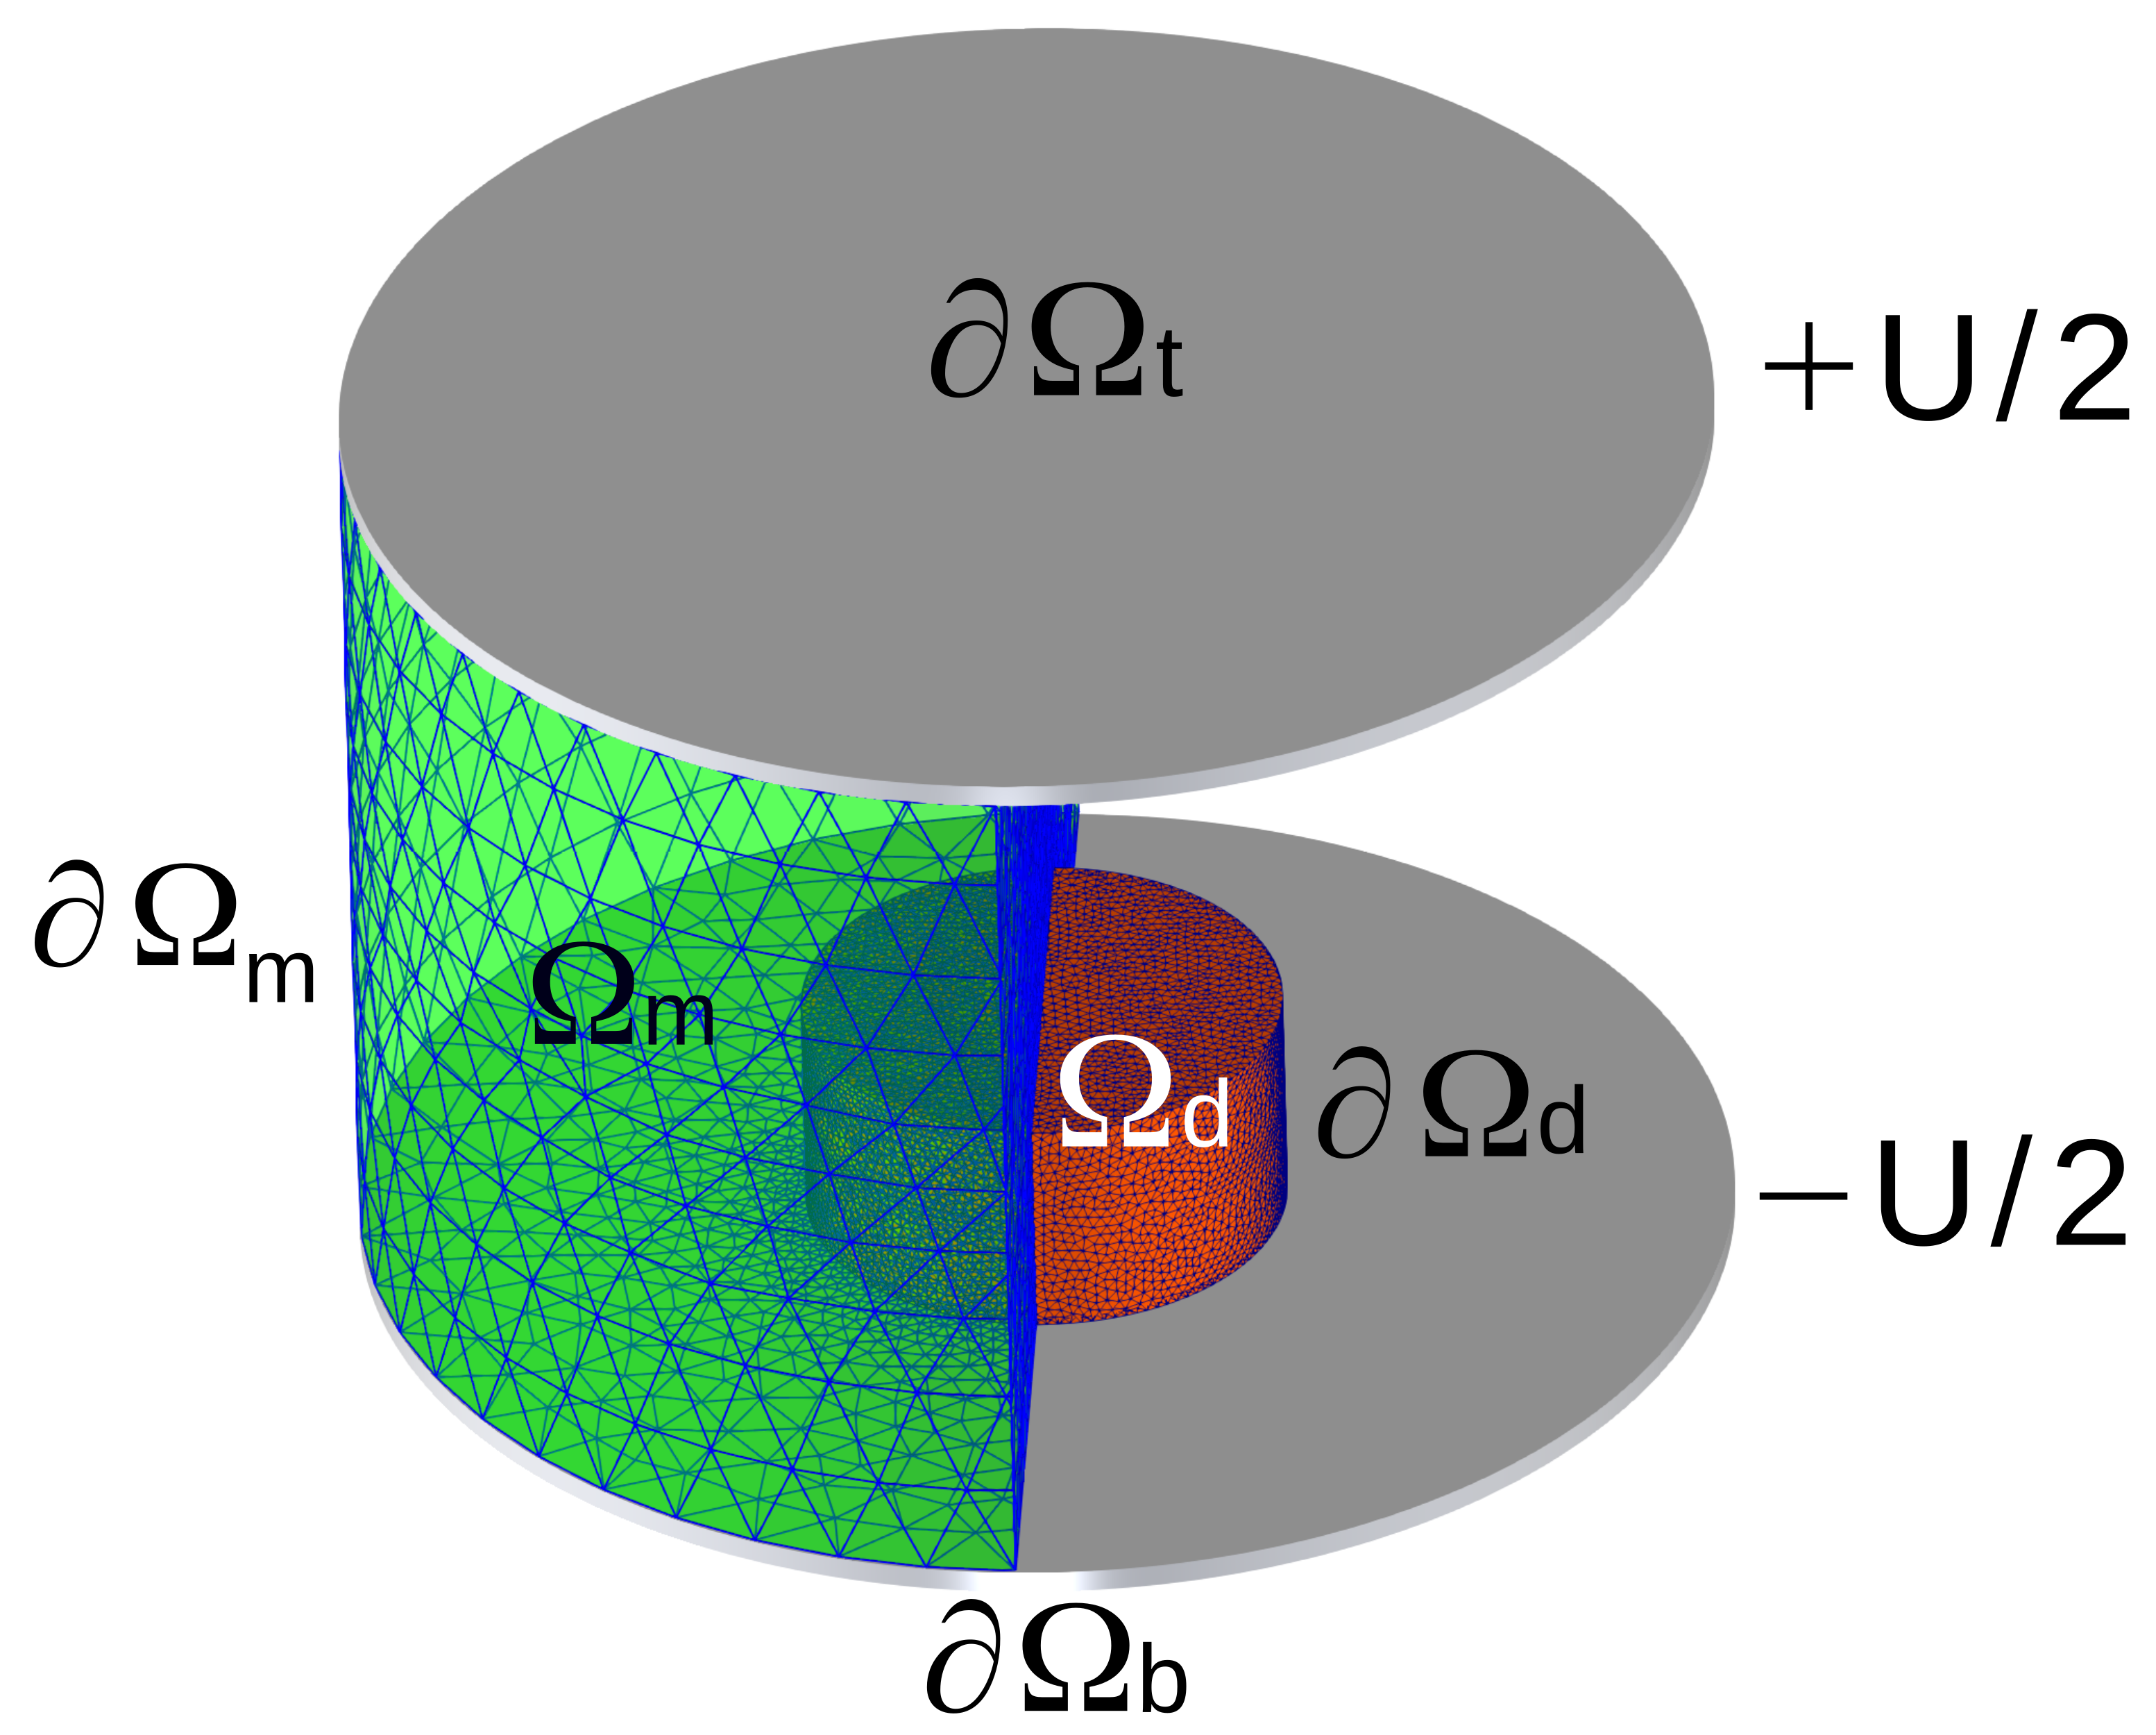
\includegraphics [width=8cm] {FigSI.png}
\caption{ \textbf{Simulation setup.}
}
\label{FigSiSetup} 
\end{figure*}
%%%%%%%%%%%%%%%%%%%%%%%%%%%%%%%%%%%%%%%%%%%%%%%%%%%%%%%%%%

\bigskip

\noindent \textbf{References}
\vspace{-0.3cm}
\bibliographystyle{unsrt}
\bibliography{bibliography}

\end{document} 
